% !TeX root = main.tex
\documentclass{beamer}

% ==================================================================
% Packages & Setup
% ==================================================================
\usepackage[utf8]{inputenc}
\usepackage{amsmath}
\usepackage{amssymb}
\usepackage{graphicx}
\usepackage{tikz}
\usefonttheme[onlymath]{serif}
\usepackage{algorithm}
\usepackage{algpseudocode}
\usepackage{xcolor}
\setbeamertemplate{bibliography item}[text]

% --- Theme Setup ---
\usetheme{Madrid}

% --- Auto-Outline at beginning of each section ---
\AtBeginSection[]{
    \begin{frame}
        \frametitle{Outline}
        \tableofcontents[currentsection, hideothersubsections, sectionstyle=show/shaded]
    \end{frame}
}

% ==================================================================
% Title Information
% ==================================================================
\title{Extending L* algorithm to Learn Syntactic Monoids}
\author{Haotian Zhang}
\date{\today}

\begin{document}

% ------------------------------------------------------------------
% Title Page
% ------------------------------------------------------------------
\frame{\titlepage}

% ------------------------------------------------------------------
% Main Outline
% ------------------------------------------------------------------
\begin{frame}
    \frametitle{Outline}
    \tableofcontents
\end{frame}


% ==================================================================
% Section 1: L* Algorithm
% ==================================================================
\section{L* algorithm}

% ------------------------------------------------------------------
% Frame: Concept of L* (Membership & Equivalence Queries)
% ------------------------------------------------------------------
\begin{frame}{L* algorithm - Learning Minimal DFA}
    \begin{block}{L* algorithm -- Learning a minimal DFA}
        For an unknown regular language $U \subseteq \Sigma^*$, find $U$'s expression using two types of queries:\cite{angluin87}
        \begin{itemize}
            \item \textbf{Membership query:} For a word $w \in \Sigma^*$, is $w \in U$?
            \item \textbf{Equivalence query:} For a DFA $\mathcal{A}$, is $L(\mathcal{A}) = U$? If the answer is no, then we can obtain a counterexample. 
        \end{itemize}
    \end{block}
    
    \begin{columns}
        \begin{column}{0.6\textwidth} 
            \centering
            % 
            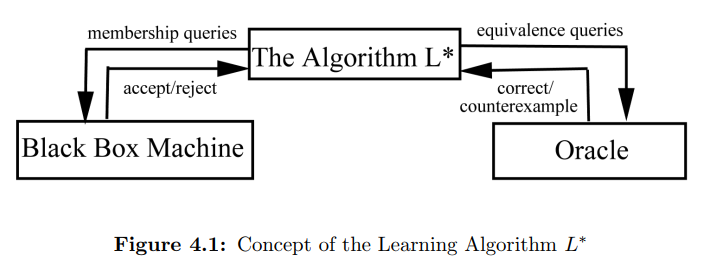
\includegraphics[width=\textwidth]{L-star-concept.png} 
        \end{column}
    \end{columns}
\end{frame}

% ------------------------------------------------------------------
% Frame: Observation Table Definition
% ------------------------------------------------------------------
\begin{frame}{L* algorithm - Observation Table }
    \begin{columns}[T]
        % --- Left Column: Definitions ---
        \begin{column}{0.6\textwidth}
            \begin{itemize}
                \item $U$ : Unknown regular language. 
                \item $\Sigma$ : Alphabet, in example it is $\{a,b\}$
                \item $I$ : Set of test states
                \item $S$ : Set of suffixes
                \item $T$: $(I \cup I \cdot \Sigma \times S) \to \{0,1\}$
                \item $OT$ : {\small Observation table, a 3-tuple } $(I,S,T)$
                \item $\text{row}(i)$: A function $\text{row} \colon I \times S \to \{0,1\}$ defined by
                $\text{row}(i)(s) = T(i,s)$.
            \end{itemize}
        \end{column}

        % --- Right Column: Example Table ---
        \begin{column}{0.6\textwidth}
            \centering
            \begin{tabular}{cc|c|c}
                &   & \multicolumn{2}{c}{$S$} \\ 
                \multicolumn{2}{c|}{} & $\epsilon$ & a \\ \hline
                & $\epsilon$ & 1 & 0 \\
                {$I$}& a          & 0 & 1 \\
                & b          & 0 & 0 \\\hline
                & aa& 1& 0 \\
                {$I\cdot \Sigma$}        & ab& 0&0\\
                & ba         & 0 & 0 \\
                & bb         & 1 & 0 \\ 
            \end{tabular}
            \par \vspace{0.2cm} 
            {\footnotesize $L = (aa + a^* b a^* b)^*$}
        \end{column}
    \end{columns}
\end{frame}

% ------------------------------------------------------------------
% Frame: Closed & Separable Definitions
% ------------------------------------------------------------------
\begin{frame}{L* algorithm - Closed \&  Separable}
    \textbf{Suffix-equivalent for $u, v \in \Sigma^{*}$: }
    $$
        u \equiv_{S} v
        \Leftrightarrow
        \text{row}(u) = \text{row}(v)
        \Leftrightarrow
        \forall s \in S,\ \text{row}(u)(s) = \text{row}(v)(s)
    $$
    \textbf{\small Separable}: \small no two distinct words in $I$ are \textbf{Suffix-equivalent}. 

    \textbf{Closed: }
    $$
        \forall i \in I , a \in \Sigma, \exists i^{\prime} \in I.ia \equiv_{S} i^{\prime}
    $$
    \centering
    \begin{tabular}{cc|c|c}
        &   & \multicolumn{2}{c}{$S$} \\ 
        \multicolumn{2}{c|}{} & $\epsilon$ & a \\ \hline
        & $\epsilon$ & 1 & 0 \\
        {$I$}& a          & 0 & 1 \\
        & b          & 0 & 0 \\ \hline
        
        & aa& 1& 0 \\
        {$I \cdot \Sigma$}& ab& 0&0\\
        & ba         & 0 & 0 \\
        & bb         & 1 & 0 \\  
    \end{tabular}
\end{frame}

% ------------------------------------------------------------------
% Frame: Acceptor Definition
% ------------------------------------------------------------------
\begin{frame}{Acceptor}
    The \textbf{Acceptor} of $(I,P,S,T)$ is a 5-tuple $\mathcal{M} = (Q,\Sigma,\delta,q_0,F)$:
    \begin{itemize}
        \item $Q = \{\text{row}(i) \mid i \in I\}$
        \item $q_0 = \text{row}(\epsilon) \in Q$
        \item $F = \{\text{row}(i) \in Q \mid \text{row}(i)(\epsilon) = 1\}$
        \item $\delta \colon Q \times \Sigma \to Q$ is the transition function.
    \end{itemize}
    \begin{block}{Construction of transition function}
        For $q \in Q, a \in \Sigma$, if $q = \text{row}(i)$ ($i \in I$) and we have
        $ia \equiv_{S} i'$, $i' \in I$, then:
        \[
            \delta(q,a) = \text{row}(i')
        \]
        The transition function $\delta$ is extended to $\delta^{*} \colon Q \times \Sigma^{*} \to Q$:
        \[
            \delta^{*}(q,w) = 
            \begin{cases}
                q & \text{if } w = \epsilon \\
                \delta(\delta^*(q,w'),a) & \text{if } w = w'a, a \in \Sigma
            \end{cases}
        \]
    \end{block}
\end{frame}

% ------------------------------------------------------------------
% Frame: Process Step 1 & 2 (Table Expansion)
% ------------------------------------------------------------------
\begin{frame}{L* algorithm - Algorithmic Process}
    1. $I:= S := \{\epsilon\}$\\
    2. If $OT$ is not closed but separable, use \textbf{membership queries} to find a
    $w^{\prime} \in I \cdot \Sigma$ such that
    $\text{row}(w^{\prime}) \ne \text{row}(w)$ for every $w \in I$.
    Add $w^{\prime}$ to $I$ and expand $I \cdot \Sigma$.
    Repeat this operation until $OT$ is separable and closed.\\
    
    \begin{columns}[T]
        % --- Left Column: Not Closed Example ---
        \begin{column}{0.45\textwidth} 
            \centering
            \begin{tabular}{cc|c|c}
                &   & \multicolumn{2}{c}{$S$} \\ 
                \multicolumn{2}{c|}{} & $\epsilon$ & a \\ \hline
                & $\epsilon$ & 1 & 0 \\
                {$I$}& a          & 0 & 1 \\ \hline
                 & \textcolor{red}{b}          & 0 & 0 \\
                {$I \cdot \Sigma$}           & aa& 1& 0 \\
                & ab& 0&0\\ 
                \multicolumn{4}{c}{} \\[-0.8em] 
                \multicolumn{4}{c}{\footnotesize Not closed}
            \end{tabular}
        \end{column}
    
        % --- Right Column: Closed Example ---
        \begin{column}{0.45\textwidth} 
            \centering
            \begin{tabular}{cc|c|c}
                &   & \multicolumn{2}{c}{$S$} \\ 
                \multicolumn{2}{c|}{} & $\epsilon$ & a \\ \hline
                & $\epsilon$ & 1 & 0 \\
                {$I$}& a          & 0 & 1 \\
                & \textcolor{red}{b}          & 0 & 0 \\\hline
                & aa& 1& 0 \\
                {$I\cdot \Sigma$}        & ab& 0&0\\
                & \textcolor{red}{ba}         & 0 & 0 \\
                & \textcolor{red}{bb}           & 1 & 0 \\ 
                \multicolumn{4}{c}{} \\[-0.8em] 
                \multicolumn{4}{c}{\footnotesize Closed}
            \end{tabular}
        \end{column}
    \end{columns}
\end{frame}


% ------------------------------------------------------------------
% Frame: Process Step 3-6 (Equivalence Query & Loop)
% ------------------------------------------------------------------
\begin{frame}{L* algorithm - Algorithmic Process}
    3. We can get an \textbf{Acceptor} (hypothesis automaton) and ask an \textbf{equivalence query} for it. \\
    4. If the answer is yes, algorithm terminates and \textbf{Acceptor} is the answer. \\
    5. If the answer is no, find a counterexample $w$ in $O(log|w|)$\cite{rivest1993inference}. Properly find the most precise suffix and add it to $S$. Now $OT$ must not be closed. \\
    6. Return to 2. 
    
    \begin{columns}
        \begin{column}{0.4\textwidth} 
            \centering
            % 
            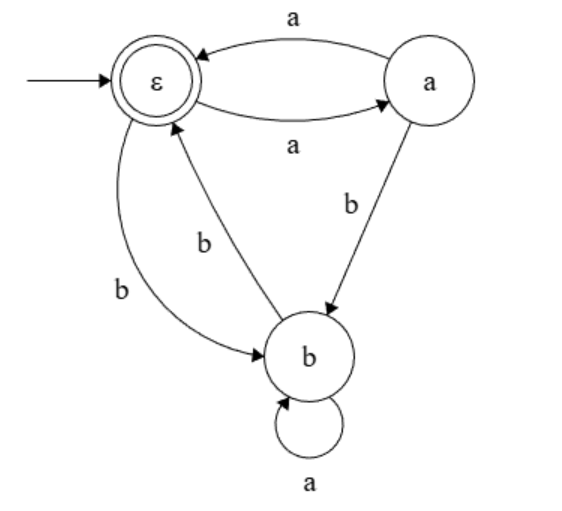
\includegraphics[width=\textwidth]{automaton.png} 
             \par \vspace{0.2cm} 
            {\footnotesize $L = (aa + a^* b a^* b)^*$}
        \end{column}
    \end{columns}
\end{frame}


% ------------------------------------------------------------------
% Frame: Process Step Summary
% ------------------------------------------------------------------
\begin{frame}{L* algorithm - Algorithmic Process}
    
    \begin{columns}
        \begin{column}{1.0\textwidth}
            \centering
            % 
            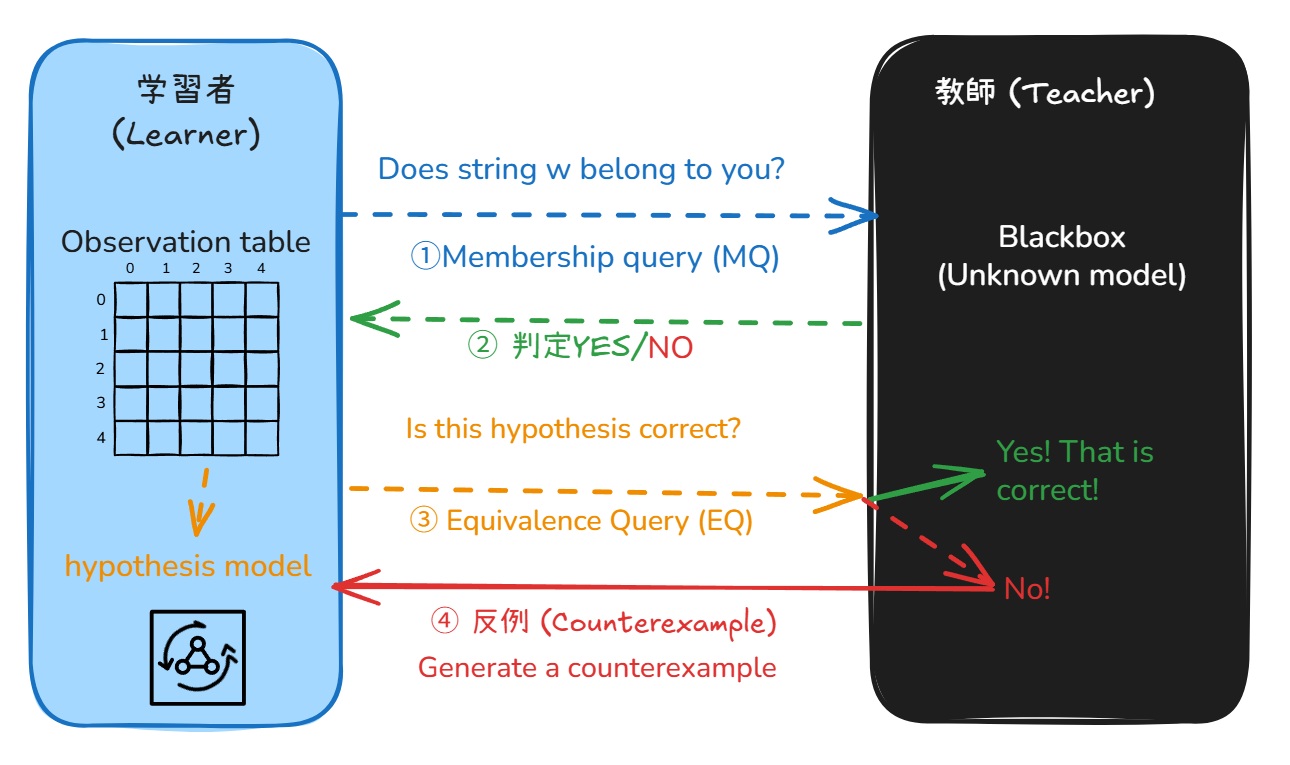
\includegraphics[width=\textwidth]{algorithm_process.png} 
             \par \vspace{0.2cm} 
        \end{column}
    \end{columns}
\end{frame}


% ==================================================================
% Section 2: Minimal DFA vs. Syntactic Monoid
% ==================================================================
\section{Minimal DFA vs. Syntactic Monoid}

% ------------------------------------------------------------------
% Frame: Definition of Minimal DFA
% ------------------------------------------------------------------
\begin{frame}{Minimal DFA}

    Let $L$ be a regular language.
    \begin{block}{Minimal DFA of L, $A_L$}
        {\small The DFA with the minimum number of states that recognizes $L$.}
        \begin{itemize}
            \item The set of states is the quotient set by the Myhill-Nerode (right) congruence:
            $$ w \equiv_{L} w' \iff \forall v \in \Sigma^*. (wv \in L \iff w'v \in L) $$
            The state set is $\Sigma^* / \equiv_L$.
        \end{itemize}
    \end{block}
\end{frame}

% ------------------------------------------------------------------
% Frame: Definition of Syntactic Monoid
% ------------------------------------------------------------------
\begin{frame}{Syntactic Monoid}
    Let $L$ be a regular language.
    \begin{block}{Syntactic Monoid of L, $M_L$}
        The monoid with the minimum order that recognizes $L$.
        \begin{itemize}
            \item The underlying set is the quotient set by the syntactic congruence:
            $$ w \cong_{L} w' \iff \forall u, v \in \Sigma^*. (uwv \in L \iff uw'v \in L) $$
            The set is $\Sigma^* / \cong_L$.
        \end{itemize}
    \end{block}
\end{frame}

% ------------------------------------------------------------------
% Frame: Comparison Example (DFA vs Monoid)
% ------------------------------------------------------------------
\begin{frame}{Minimal DFA vs. Syntactic Monoid}
    \textbf{Example:} Let $L = (ab)^* \subseteq \{a, b\}^*$.
    \vspace{-0.4em} 
    \begin{columns}
        % --- Left: Minimal DFA ---
        \begin{column}{0.48\textwidth} 
            \centering
            \textbf{Minimal DFA $A_L$} 
            % 
            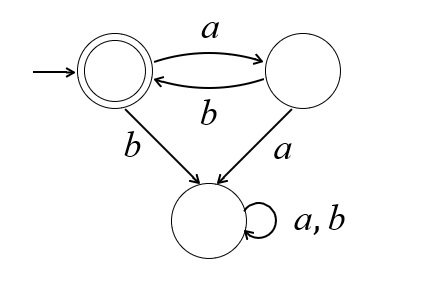
\includegraphics[width=\textwidth]{1.png} 
        \end{column}
    
        % --- Right: Syntactic Monoid ---
        \begin{column}{0.48\textwidth} 
            \centering
            \textbf{Syntactic Monoid $M_L$} 
            (Right Cayley Graph) 
            % 
            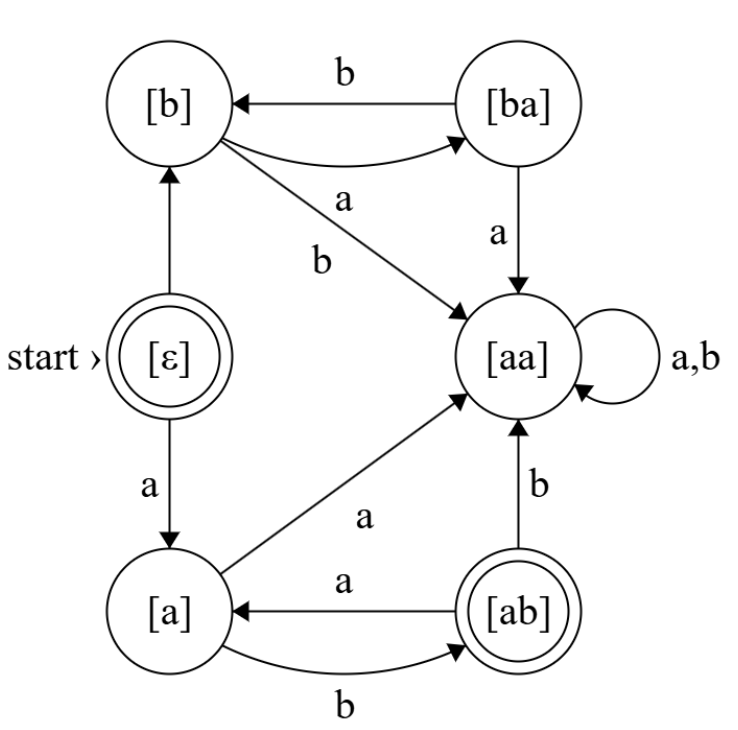
\includegraphics[width=\textwidth]{2.png} 
        \end{column}
    \end{columns}
\end{frame}

% ------------------------------------------------------------------
% Frame: Motivation
% ------------------------------------------------------------------
\begin{frame}{Motivation -- Why Learn Syntactic Monoids?}
    \begin{block}{Language Behavior and Algebraic Structure}
        \begin{itemize}
            \item A minimal DFA identifies words with the same behavior
            under all right contexts.
            \item The syntactic monoid distinguishes words using both
            left and right contexts, and records how their classes multiply.
        \end{itemize}
    \end{block}
    \begin{block}{A Structure for Property Checking}
        Many language properties have algebraic characterizations,
        including star-freeness, commutativity, and being a group language.
        Learning $M_L$ provides a common structure for these checks.
    \end{block}
    {\small With $n=|A_L|$ and $M=|M_L|$, we have $n\leq M\leq n^n$
    \cite{holzer2004deterministic}. The richer structure can be much larger.}
\end{frame}


% ------------------------------------------------------------------
% Frame: Motivation
% ------------------------------------------------------------------
\begin{frame}{Motivation -- Example: Star-freeness}
    \begin{block}{Star-free Languages}
        Star-free expressions use union, concatenation, and complement,
        without the Kleene star. For $\Sigma=\{a,b\}$, $(ab)^*$ is star-free:
        $$
        (ab)^*=
        \overline{
        b\Sigma^*\cup\Sigma^*a
        \cup\Sigma^*(aa\cup bb)\Sigma^*
        },
        \qquad \Sigma^*=\overline{\emptyset}.
        $$
    \end{block}
    \begin{block}{Algebraic Characterization}
        $$
        L\text{ is star-free}
        \Longleftrightarrow M_L\text{ is aperiodic}.
        \quad \cite{SCHUTZENBERGER1965190}
        $$
        Equivalently, $A_L$ is counter-free \cite{thomas2005applied}.
        In $M_L$, every element's powers eventually stabilize:
        $$
        \forall m\in M_L,\quad \exists r\geq 1:\quad m^r=m^{r+1}.
        $$
    \end{block}
    {\small Property-checking costs exclude the cost of acquiring the monoid.}
\end{frame}

% ------------------------------------------------------------------
% Frame: Three Learning Routes (inserted before the original learning-problem slide)
% ------------------------------------------------------------------
\begin{frame}{Motivation -- Three Learning Routes}
    \begin{block}{The Conventional Route}
        \[
        \text{Queries}\xrightarrow{\text{L*}} A_L
        \mathrel{\tikz[baseline=-0.6ex]{
            \draw[dashed,->,line width=0.45pt] (0,0)--(3.2,0);
            \node[above=4pt,inner sep=0pt,font=\scriptsize] at (1.6,0)
                {local construction};
        }} M_L
        \]
        {\small Only the L* stage uses active learning. Once $A_L$ is exact,
        it determines $M_L$ without further queries~\cite{froidure1997algorithms}.}
    \end{block}

    \begin{block}{The Post-check Route}
        \[
        \text{Queries}\xrightarrow{\text{L*}} A_L
        \xrightarrow{\text{Monoid Consistency Check}} M_L
        \]
    \end{block}

    \begin{block}{The Promote-to-$P$ Route}
        \[
        \text{Queries}\xrightarrow{\text{L*}} M_L
        \]
    \end{block}

    {\footnotesize Solid arrows indicate active learning steps; the dashed arrow
    indicates local construction after learning.}
\end{frame}

% ------------------------------------------------------------------
% Frame: Exact and Sample-based Equivalence Queries
% ------------------------------------------------------------------
\begin{frame}{Motivation - About the Equivalence Query}
    \footnotesize
    \begin{block}{Ideal Equivalence Query}
        \begin{itemize}
            \item An exact EQ decides whether $L(\mathcal{A})=U$; otherwise it
            returns a counterexample.
            \item After a successful exact EQ, a $P$-only Monoid Consistency
            refinement cannot change the recognized language. No new EQ is needed.
        \end{itemize}
    \end{block}
    \vspace{-0.5em}

    \begin{block}{Sample-based EQ Approximation}
        \begin{itemize}
            \item Compare the hypothesis and black box on random labeled words.
            A mismatch is a counterexample; passing the sample gives only a
            probabilistic approximation \cite[Sec.~4]{angluin87}.
            \item A later Monoid Consistency Check may expose a language
            counterexample missed by sampling. Then a new EQ is needed.
        \end{itemize}
    \end{block}
    \vspace{-0.5em}

    \begin{alertblock}{Research Hypothesis}
        With exact MQs and a fixed sampling budget, can fewer approximate EQs
        allow more samples per test and improve confidence?
    \end{alertblock}
\end{frame}

% ------------------------------------------------------------------
% Frame: Research Goals
% ------------------------------------------------------------------
\begin{frame}{Motivation -- Our Goal}
    \begin{block}{Goal 1: Algorithm and Correctness}
        Extend L* to \textbf{actively learn the right Cayley graph} of the
        syntactic monoid, and prove that the algorithm is correct under
        exact membership and equivalence queries.
    \end{block}

    \begin{block}{Goal 2: Strategy Comparison}
        Use concrete experiments to compare the strengths and weaknesses of
        \textbf{Post-check} and \textbf{Promote-to-$P$}, and identify which
        language classes favor each strategy.
    \end{block}
\end{frame}
% ==================================================================
% Section 3: Idea of Learning Syntactic Monoid
% ==================================================================
\section{Idea of Learning Syntactic Monoid}

% ------------------------------------------------------------------
% Frame: Extended Observation Table
% ------------------------------------------------------------------
\begin{frame}{Extended Observation Table}
    Let $U\subseteq\Sigma^*$ be regular, with membership function
    $\chi(w)=1$ iff $w\in U$.
    \begin{itemize}
        \item $I$: a prefix-closed set of state representative strings.
        \item $P$: left contexts. \qquad $S$: right contexts.
        \item $\epsilon\in I\cap P\cap S$.
    \end{itemize}
    The observation table is $OT=(P,I,S,T)$, where
    $$
    \begin{aligned}
        T&:P\times(I\cup I\cdot\Sigma)\times S\to\{0,1\},\\
        T(p,w,s)&=\chi(pws).
    \end{aligned}
    $$
    \begin{block}{Two Row Functions}
        For $w\in\Sigma^*$:
        $$
        \begin{aligned}
            \text{row}(w)=\text{row}_{P,S}(w)&=(\chi(pws))_{(p,s)\in P\times S},\\
            \text{row}_S(w)&=(\chi(ws))_{s\in S}.
        \end{aligned}
        $$
    \end{block}
\end{frame}

% ------------------------------------------------------------------
% Frame: Equivalence, Closedness and Separability
% ------------------------------------------------------------------
\begin{frame}{Observed Equivalence and Table Conditions}
    \begin{block}{Two Equivalence Relations}
        For $u,v\in\Sigma^*$:
        $$
        \begin{aligned}
            u\equiv_{\mathrm{status}}v
                &\Longleftrightarrow \text{row}(u)=\text{row}(v),\\
            u\equiv_S v
                &\Longleftrightarrow \text{row}_S(u)=\text{row}_S(v).
        \end{aligned}
        $$
        Since $\epsilon\in P$, status equivalence implies suffix equivalence.
    \end{block}
    \begin{block}{Closedness and Separability}
        \textbf{Closed:}
        $$
        \forall t\in I\cdot\Sigma,\quad
        \exists i\in I:\ t\equiv_{\mathrm{status}}i.
        $$
        \textbf{Separable:} Distinct strings in $I$ have distinct full rows.
        If closedness fails, add a boundary string with a new row to $I$.
    \end{block}
\end{frame}

% ------------------------------------------------------------------
% Frame: Extended Observation Table Example
% ------------------------------------------------------------------
\begin{frame}{Extended Observation Table -- Example}
    $U=(ab)^*$, \qquad $\Sigma=\{a,b\}$.
    \vspace{0.4em}
    \begin{columns}[T,onlytextwidth]
        \begin{column}{0.55\textwidth}
            \centering
            \small
            \setlength{\tabcolsep}{4pt}
            \renewcommand{\arraystretch}{1.05}
            \begin{tabular}{cc|cc|cc}
                & $w$ & \multicolumn{4}{c}{$P\times S$}\\
                & & \multicolumn{2}{c|}{\textcolor{blue}{$p=\epsilon$}}
                  & \multicolumn{2}{c}{$p=a$}\\
                & $s$ & \textcolor{blue}{$\epsilon$}
                      & \textcolor{blue}{$b$} & $\epsilon$ & $b$\\ \hline
                & $\epsilon$ & \textcolor{blue}{1} & \textcolor{blue}{0} & 0 & 1\\
                $I$ & $a$    & \textcolor{blue}{0} & \textcolor{blue}{1} & 0 & 0\\
                & $b$ & \textcolor{blue}{0} & \textcolor{blue}{0}
                    & \textcolor{red}{1} & \textcolor{red}{0}\\ \hline
                & $aa$ & \textcolor{blue}{0} & \textcolor{blue}{0} & 0 & 0\\
                $I\Sigma\setminus I$ & $ab$
                    & \textcolor{blue}{1} & \textcolor{blue}{0} & 0 & 0\\
                & $ba$ & \textcolor{blue}{0} & \textcolor{blue}{0} & 0 & 1\\
                & $bb$ & \textcolor{blue}{0} & \textcolor{blue}{0} & 0 & 0\\ \hline
            \end{tabular}
            \par\vspace{0.4em}
        \end{column}
        \begin{column}{0.43\textwidth}
            \small
            \begin{itemize}
                \item $P=\{\epsilon,a\}$: left contexts.
                \item $S=\{\epsilon,b\}$: right contexts.
                \item $I=\{\epsilon,a,b\}$: state representatives.
                \item $I\Sigma$: one-letter extensions of $I$.
            \end{itemize}
            \textbf{Reading a row:}
            $$
            \text{row}(b)=(\textcolor{blue}{0,0},\textcolor{red}{1,0}).
            $$
            $$
            \text{row}_S(b)=(\textcolor{blue}{0,0}).
            $$
            The full row uses all columns; $\text{row}_S$ uses only
            \textcolor{blue}{blue columns} ($p=\epsilon$).
        \end{column}
    \end{columns}
    \vspace{0.5em}
    {\small Each cell records $\chi(pws)$.
    For example, $T(a,b,\epsilon)=\chi(ab)=1$.}
\end{frame}

% ------------------------------------------------------------------
% Frame: Hypothesis Acceptor
% ------------------------------------------------------------------
\begin{frame}{Hypothesis Acceptor}
    For a closed, separable table, construct
    $\mathcal{M}=(Q,\Sigma,\delta,q_0,F)$:
    \begin{itemize}
        \item $Q=\{\text{row}(i)\mid i\in I\}$.
        \item $q_0=\text{row}(\epsilon)$.
        \item $F=\{\text{row}(i)\mid i\in I,\ \chi(i)=1\}$.
    \end{itemize}
    \begin{block}{One-letter Right Transitions}
        For $i\in I$ and $a\in\Sigma$, choose $i'\in I$ with
        $ia\equiv_{\mathrm{status}}i'$. Define
        $$
        \delta(\text{row}(i),a)=\text{row}(i').
        $$
        Closedness provides $i'$, and separability makes it unique.
    \end{block}
    An equivalence query checks whether $L(\mathcal{M})=U$.
\end{frame}

% ------------------------------------------------------------------
% Frame: Right Consistency and Refinement
% ------------------------------------------------------------------
\begin{frame}{Right Consistency}
    \begin{block}{Definition}
        For all $i,j\in I$ and $a\in\Sigma$:
        $$
        i\equiv_S j\quad\Longrightarrow\quad ia\equiv_S ja.
        $$
    \end{block}
    \begin{block}{Refinement}
        A violation gives $i\equiv_S j$ and some $a\in\Sigma$, $s\in S$ with
        $$
        \chi(ias)\neq\chi(jas).
        $$
        Add the distinguishing suffix:
        $$
        S\leftarrow S\cup\{as\}.
        $$
        Refill the table and recheck closedness and right consistency.
    \end{block}
\end{frame}

% ------------------------------------------------------------------
% Frame: Monoid Consistency and Refinement
% ------------------------------------------------------------------
\begin{frame}{Monoid Consistency}
    \begin{block}{Definition}
        For $v\in I$ and $t\in I\cdot\Sigma$, require:
        $$
        \begin{aligned}
            t\equiv_{\mathrm{status}}v
            \quad\Longrightarrow\quad
            &\forall i\in I,\ \forall s\in S,\\
            &\chi(its)=\chi(ivs).
        \end{aligned}
        $$
    \end{block}
    \begin{block}{Refinement}
        A violation gives a left context $i\in I$ and $s\in S$ with
        $\chi(its)\neq\chi(ivs)$. Add
        $$
        P\leftarrow P\cup\{i\}.
        $$
        This separates the rows of $t$ and $v$. Refill and recheck the table.
    \end{block}
    {\small With separability, closedness, right consistency and exact language equivalence,
    monoid consistency certifies the right Cayley graph of $M_U$.}
\end{frame}

% ------------------------------------------------------------------
% Frame: Two Learning Strategies
% ------------------------------------------------------------------
\begin{frame}{Two Learning Strategies}
    Both strategies start with $I=P=S=\{\epsilon\}$.
    \begin{block}{Post-check}
        Introduce left contexts on demand after language equivalence.
        \begin{itemize}
            \item A monoid-consistency violation adds its witness to $P$.
            \item Stop when language equivalence and monoid consistency hold.
        \end{itemize}
    \end{block}
    \begin{block}{Promote-to-$P$}
        Whenever closedness adds $t$ to $I$, also add $t$ to $P$:
        $$
        I\leftarrow I\cup\{t\},\qquad P\leftarrow P\cup\{t\}.
        $$
        Thus $I\subseteq P$: full-row equality already checks every left
        context required by monoid consistency. No separate check is needed.
    \end{block}
\end{frame}

% ------------------------------------------------------------------
% Frame: Post-check Process
% ------------------------------------------------------------------
\begin{frame}{Algorithm -- Post-check}
    \begin{enumerate}
        \item Initialize $I=P=S=\{\epsilon\}$.
        \item Fill the table using MQs. Add new boundary rows to $I$ and
        repair right-consistency violations by extending $S$.
        Repeat until the table is closed and right consistent.
        \item Construct $\mathcal{M}$. Ask an EQ unless language equivalence
        is already confirmed.
        \item If the EQ returns a counterexample, use Rivest--Schapire
        refinement to add a distinguishing suffix to $S$. Return to step 2.
        \item After language equivalence, check monoid consistency.
        On failure, add the distinguishing left context to $P$
        and return to step 2.
        \item If monoid consistency holds, return $\mathcal{M}$.
    \end{enumerate}
    \vspace{0.3em}
    {\small A refinement of $P$ alone can reuse the previous language
    equivalence result. A change to $S$ requires another EQ.}
\end{frame}

% ------------------------------------------------------------------
% Frame: Promote-to-P Process and Correctness
% ------------------------------------------------------------------
\begin{frame}{Algorithm -- Promote-to-$P$}
    \begin{enumerate}
        \item Initialize $I=P=S=\{\epsilon\}$.
        \item Fill the table using MQs. For each new boundary row,
        add its string to both $I$ and $P$. Repeat until closed.
        \item Check right consistency. On a violation, add the distinguishing
        suffix $as$ to $S$ and return to step 2.
        \item Construct $\mathcal{M}$ and ask an EQ.
        On a counterexample, add a distinguishing suffix to $S$
        using Rivest--Schapire refinement and return to step 2.
        \item If the EQ succeeds, return $\mathcal{M}$.
        The invariant $I\subseteq P$ ensures monoid consistency.
    \end{enumerate}
    \begin{alertblock}{Correctness}
        For a regular target language and exact MQs and EQs,
        both strategies terminate and return the right Cayley graph
        of its syntactic monoid.
    \end{alertblock}
\end{frame}

% ------------------------------------------------------------------
% Frame: Comparison of the two learning strategies
% ------------------------------------------------------------------
\begin{frame}{Post-check vs. Promote-to-$P$}
    \footnotesize
    \begin{columns}[T,onlytextwidth]
        \begin{column}{0.47\textwidth}
            \begin{block}{Post-check}
                \begin{itemize}
                    \item Adds a distinguishing prefix to $P$ only when needed.
                    \item Runs a separate Monoid Consistency Check.
                    \item Keeps the table smaller and may use fewer table MQs.
                    \item May require more EQs.
                \end{itemize}
            \end{block}
        \end{column}
        \begin{column}{0.47\textwidth}
            \begin{block}{Promote-to-$P$}
                \begin{itemize}
                    \item Adds every new representative in $I$ to $P$ immediately.
                    \item Creates a larger observation table and may use more table MQs.
                    \item Needs no separate Monoid Consistency Check.
                    \item May require fewer EQs.
                \end{itemize}
            \end{block}
        \end{column}
    \end{columns}

    \vspace{0.4em}
    \begin{alertblock}{If EQs Are Approximated by Sampling}
        With fixed samples per EQ, more EQs use more sampled MQs.
        With a fixed total sampling budget, fewer EQs allow more samples
        per test and may improve confidence.
    \end{alertblock}
\end{frame}


% ==================================================================
% Section 5: Future Work
% ==================================================================
\section{Future work}

% ------------------------------------------------------------------
% Frame: Future Tasks
% ------------------------------------------------------------------
\begin{frame}{Summary and Future Work}
    \begin{block}{Summary}
        \begin{itemize}
            \item Extended the L* observation table with left and right
            contexts to actively learn the \textbf{Syntactic Monoid}.
            \item Proved correctness using \textbf{Right Consistency} and
            \textbf{Monoid Consistency}: for regular targets and exact MQs
            and EQs, the algorithm terminates with the right Cayley graph.
            \item Presented two strategies: \textbf{Post-check} and
            \textbf{Promote-to-$P$}, differing in when left contexts are added.
        \end{itemize}
    \end{block}

    \begin{block}{Future Work}
        \begin{itemize}
            \item Design experiments on different language classes,
            including star-free languages and group languages.
            \item Explore which language structures favor each strategy.
            \item Compare both strategies with the traditional route:
            $\text{L*}\to A_L\to M_L$.
        \end{itemize}
    \end{block}
\end{frame}

% ==================================================================
% References
% ==================================================================
\begin{frame}[allowframebreaks] 
    \frametitle{References}
    
    \bibliographystyle{IEEEtran}
    \bibliography{reference} 
\end{frame}

% ==================================================================
% Backup Slides: Correctness Details
% ==================================================================
\appendix

\begin{frame}{Path Representative Function}
    \begin{block}{Definition of Representative Function}
        Assume that the observation table is closed.
        Define the Path representative function $\rho:\Sigma^*\to I$ recursively as follows:
        \[
        \rho(\epsilon)=\epsilon,
        \]
        and for every $x = ya(x,y\in\Sigma^*, a\in\Sigma)$ and $\rho(y) = i (i\in I)$. Then because of closedness:
        \[
        \exists u \in I. ia \equiv_{status} u.
        \]
        and $\rho(ya) = \rho(x) = u$. 
    \end{block}

    \begin{alertblock}{Intuition}
        The path representative labels the state reached after reading $w$:
        $
        \delta^*(q_0,w)=\text{row}(\rho(w)).
        $
        Its status equivalence to $w$ is a proved property, not part of
        the recursive definition.
    \end{alertblock}
\end{frame}

% ==================================================================
% Slide: Proposition 2 series
% ==================================================================

\begin{frame}{Proposition 2.2 - 2.3}
    \begin{block}{Assumption}
        Assume $\epsilon\in I\cap P\cap S$, prefix-closed $I$, and a
        separable, closed, right-consistent table. The hypothesis passes
        an exact EQ, so $L(\mathcal{M})=U$.
    \end{block}

    \begin{block}{Propositions}
        \begin{itemize}
            \item Proposition 2.2:  
            \[
                \forall w \in \Sigma^*, w \equiv_S \rho(w).
            \]
            \item Proposition 2.3: 
             \[
                \forall u,v \in \Sigma^*. u \equiv_S v \Rightarrow (\forall y \in \Sigma^*. uy \in U \iff vy \in U). 
            \]
        \end{itemize}
    \end{block}
\end{frame}

% ==================================================================
% Slide: Proposition 2 series
% ==================================================================

\begin{frame}{Proposition 2.4}
    \begin{block}{Proposition}
        \[
            \forall u,v \in \Sigma^*. u \equiv_{status} v \Rightarrow (\forall a \in \Sigma. ua \equiv_{status} va).
        \]
    \end{block}
    \begin{block}{Proof}
        Assume that $u \equiv_{status} v$, therefore we have:
         \[
            \forall p\in P,s\in S. \chi(p\cdot u \cdot s) = \chi(p\cdot v \cdot s).
        \]
        Thus, for every $p \in P$, $pu \equiv_{S} pv$.
        By Proposition 2.3, for every $z \in \Sigma^*$ we have $puz \in U \iff pvz \in U$.
        So take $z = as$, where $a \in \Sigma$ and $s \in S$, we have $puas \in U \iff pvas \in U$.
        Therefore,
        \[
            ua \equiv_{status} va.
        \]
    \end{block}
\end{frame}

\begin{frame}{Proposition 2.5 - 2.6}
    \begin{block}{Propositions}
       \begin{itemize}
            \item Proposition 2.5:  
            \[
                \forall u \in \Sigma^*, u \equiv_{status} \rho(u).
            \]
            This can be easily proved by induction based on the conclusion in Proposition 2.4.
            \item Proposition 2.6: 
             \[
                \forall u,v \in \Sigma^*. u \equiv_{status} v \iff \delta^*(q_0,u) = \delta^*(q_0,v).
            \]
            Therefore, under the assumption we mentioned, two status-equivalent words must go to the same state. 
        \end{itemize}
    \end{block}
\end{frame}

\end{document}
